\subsection*{Introduction}

    When running an optimization solver on a set  $\Pset$ of problems, it is
    usual to record information of interest --- such as CPU time, number of
    functions evaluations, number of iterations, or others --- which we will
    reference as \emph{cost}. This process is called Benchmark.

    Benchmarking an optimization software has been a necessity and some works
    has showed that uncovered deficiencies in the software and has generally led
    to software
    improvements~\cite{url:mittelmann,Mittelmann:1999fb,Dolan:2006kl}.
    In this sense, \textcite{Dolan:2002du} developed a tool to compare
    optimization solvers benchmarks: the Performance Profile.

    The Performance Profile is a means to evaluate and compare the performance
    of a set of solvers $\Sset$ on a test set $\Pset$. It is presented as a
    graphic that shows the cumulative distribution function of different solvers
    performances, according to the chosen cost metric, for a given set of
    problem instances.

    For each
    problem $p \in \Pset$ and solver $s \in \Sset$, let $t_{ps}$ be the
    cost required to solve problem $p$ by solver $s$ and
    \begin{align*}
      r_{ps} = \frac{t_{ps}}{\min\{t_{ps}: s \in \Sset\}}
    \end{align*}
    be the performance ratio of solver $s$ for the problem $p$ when compared
    with the best performance by any solver on this problem.
    As a convention, we set $r_{ps}$ to a large value, let's say $r_{\max}$, if
    the solver $s$ does not solve the problem $p$.

    The probability of a solver $s \in \Sset$  to solve one problem within a
    factor $\tau \in \mathds{R}$ of the best performance ratio is the function
    \begin{align*}
      \rho_s(\tau) = \frac{| \{p \in \Pset: r_{ps} \leq \tau\} |}{| \Pset |}.
    \end{align*}
    For a given $\tau$, the best solver is the one with the highest value for
    $\rho_s(\tau)$, that is, the one with the highest probability to solve the
    problem.
    The value $\rho_s(\tau)$ gives the percentage of problems solved by
    algorithm $s$ with a cost at most $\tau$ times worst than the best
    algorithm. $\rho_s(1)$ is the percentage of problems solved as fast as the
    fastest algorithm, which gives the efficiency of solver $s$.
    On the other hand
    \[\displaystyle \lim_{\tau\rightarrow r^-_{\max}} \rho_s(\tau)\]
    is the total percentage of problems solved by solver $s$, in
    other words, the robustness of solver $s$.

\subsection*{Motivation}

    To facilitate the reproduction of data set analysis, such as the
    benchmarking of solvers analysis provided by \citeauthor{Dolan:2002du}'s
    performance profile, it is important to have an open source tool that handle
    the production of plots.

    Performance profile has been, over the years, the most used benchmark
    comparison tool used in optimization. Nevertheless, the production of such
    analysis is sometimes a dull task, that can lead a researcher to waste a lot
    of time and effort that should have been spent in developing the solver
    itself.

    There are third part implementations to generate the Performance Profile.
    The same group that created the Performance Profile released a MATLAB
    script in their website~\cite{url:cops}. There is also a module written by
    Michal Friedlander inside
    NLPy~\cite{url:NLPy} that is able to produce the Performance Profile.
    However, there are features that some users need that those softwares did
    not implement.

    We thus designed a straightforward tool that allows one to create
    performance profile pictures in a fast and easy manner.

    In addition, this tool would allow \LaTeX\ users, a group in which almost
    all optimization community is included, to generate performance profile
    plots within \LaTeX\ environment, and thus to get a better typographic
    result other than simple including raster  images.

    With these two main goals in mind, we developed and implemented perprof-py
    in Python 3 with internationalization features and direct \LaTeX\
    integration.

\subsection*{Implementation and architecture}

    The software was implemented as a Python 3 package
    and organized
    to allow addition of new backends --  see Figure~\ref{fig:uml}.
    Users have a command line interface to use out of the box,
    however one can also use the package in their own software.

    \begin{figure}[!htb]
      \centering
      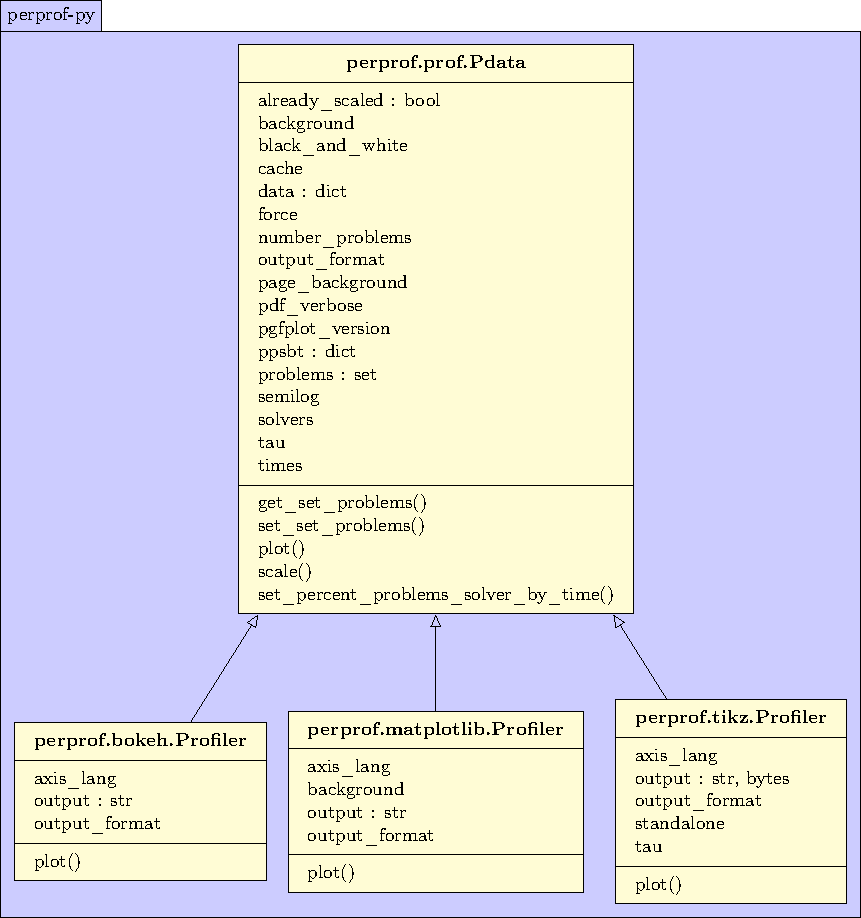
\includegraphics[width=0.45\textwidth]{uml/uml.pdf}
      \caption{UML of perprof}
      \label{fig:uml}
    \end{figure}

    The implementation is very straightforward. The algorithm:
    \begin{enumerate}
      \item parses the options passed as arguments, creating a
        structure with all the information;
      \item parses and process the input files, using the definition
        of the performance function to create the data to be plotted;
      \item uses the chosen backend to plot the data.
    \end{enumerate}

\subsection*{Input}

    For each solver to be compared in the benchmark, one must write a file in
    the following manner:

    \begin{verbatim}
---
YAML information
---
Problem01 exit01 time01
Problem02 exit02 time02
    \end{verbatim}

    In the YAML information one can set the name of the solver and some
    flags for perprof-py.
    Each line beyond that has 3 columns. The columns meaning, in order, are:
    \begin{itemize}
      \item The name of the problem;
      \item Exit flag;
      \item Cost measure -- for instance, elapsed time.
    \end{itemize}

\subsection*{Parsing process and output}

    To use perprof-py, the user needs to issue a command of the type
\begin{verbatim}
$ perprof OPTIONS BACKEND FILES
\end{verbatim}
    where
    \begin{itemize}
      \item FILES are the input files described in the previous section. At
        least two files input are required;
      \item BACKEND is one of the options \verb+--tikz+, \verb+--mp+,
        \verb+--bokeh+ or
        \verb+--raw+, which represents whether the user wants to use
        Tikz/PGFPLOTS, MatplotLib, Bokeh, or simply printing the performance
        ratios, respectively;
      \item OPTIONS are varied arguments that can be passed to perprof-py to
        customize the graphics or modify the performance functions. Some
        noteworthy options are
        \begin{itemize}
          \item \verb+--semilog+: the natural logarithmic scale is used on the
          abscissa axis;
          \item \verb+--success STR+: \verb+STR+ is a comma separated string
            of keys that was considered  \emph{success} by the solver;
          \item \verb+--black-and-white+: perprof-py creates the plots using
            only line styles and it colors them in black;
          \item \verb+--subset FILE+: perprof-py considers only the subset problems listed in \verb+FILE+, while creating the performance functions.
        \end{itemize}
    \end{itemize}
    In order to demonstrate such OPTIONS, Figures
    \ref{fig:example1}-\ref{fig:example4} show some examples of  performance
    profile graphics.
    Figure \ref{fig:example1} shows the performance profile graphic with default
    options. Note that the lines are clumped due to the maximum time allowed
    in the solver.
    \begin{figure}[!ht]
      \centering
      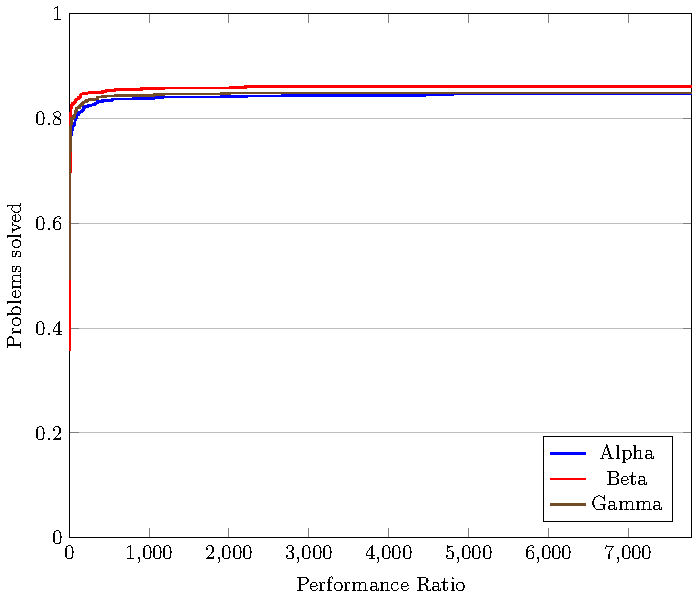
\includegraphics[width=0.4\textwidth]{plots/abc.pdf}
      \caption{Example of performance profile with default options.}
      \label{fig:example1}
    \end{figure}
    Figure \ref{fig:example2} shows the performance profile using the semilog
    option, which plots the graphic using a log scale on the abscissa.
    \begin{figure}[!ht]
      \centering
      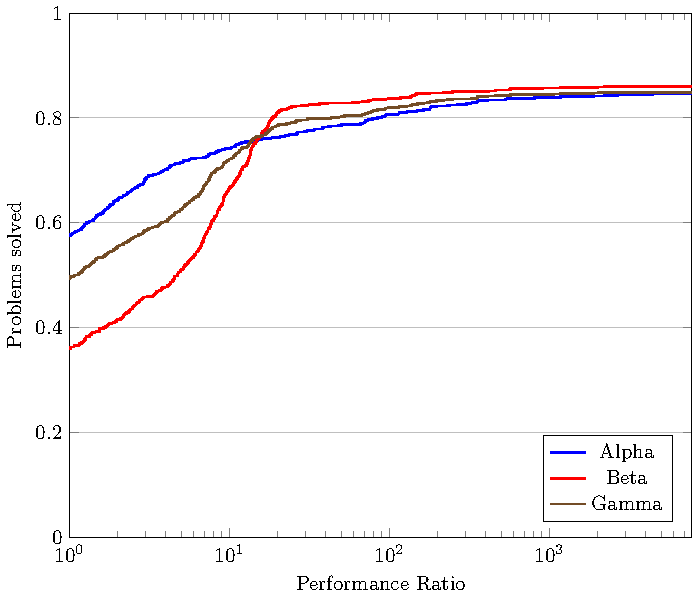
\includegraphics[width=0.4\textwidth]{plots/abc-semilog.pdf}
      \caption{Example of performance profile with semilog option.}
      \label{fig:example2}
    \end{figure}
    Figure \ref{fig:example3} shows the performance profile using also the black
    and white option, which gives a printer-friendly graphic.
    \begin{figure}[!ht]
      \centering
      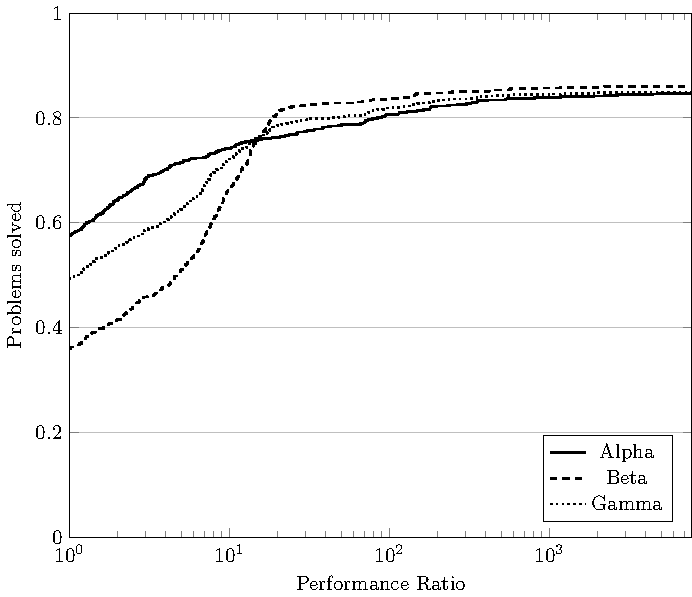
\includegraphics[width=0.4\textwidth]{plots/abc-semilog-bw.pdf}
      \caption{Example of performance profile with semilog and black and white
        options.}
      \label{fig:example3}
    \end{figure}
    Fugre \ref{fig:example4} shows the performance profile using the subset
    option in addition to previous options. In this case, we selected around 120
    problems, put their names in a file, and passed the file with the option.
    This limits the comparison to only those files.
    \begin{figure}[!ht]
      \centering
      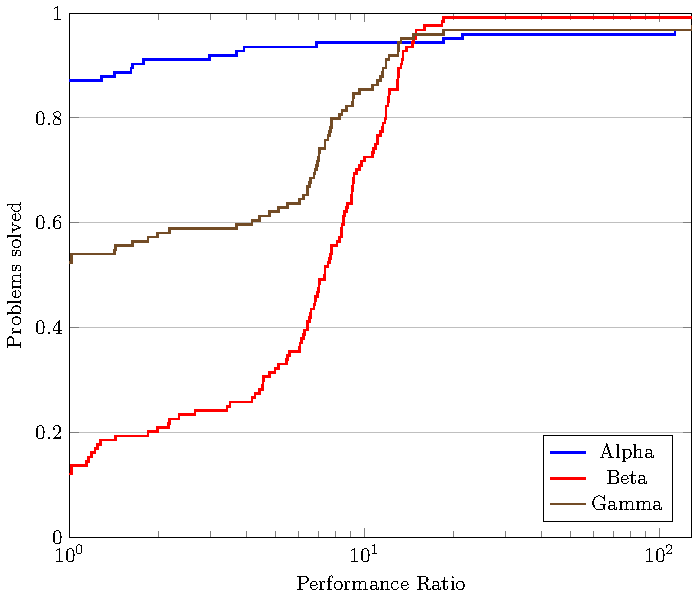
\includegraphics[width=0.4\textwidth]{plots/abc-semilog-hs.pdf}
      \caption{Example of performance profile with semilog and subset options.}
      \label{fig:example4}
    \end{figure}

\subsection*{Quality control}

    The code is tested using unit tests that verify if wrong input information
    is captured. These tests are run automatically on Travis CI
    \cite{url:travis}, for Python 3.3 and 3.4.
    Functional tests related to the graphics must be done manually.
    These tests use artifial solver information accessible using \verb+--demo+
    as argument in the perprof-py call. The user can run a script that makes
    several of these graphics in various formats by entering the folder
    \verb+perprof/examples+ relative to the package folder, and running
\begin{verbatim}
./make-examples.sh
\end{verbatim}
    The folder \verb+plots+ will contain the outputs in formats PNG, PDF and HTML.
